
\subsection{Geometry, Material Properties and Mesh}

Due to the lack of data about thermal material properties of CTD-101K and S2-glass at the cryogenic temperatures, it is assumed in this thesis that the region outside of the composite strand is homogenised and represented by G10. G10 is a material widely known and applied in the superconducting magnets design community. Its material properties are presented in Appendix~\ref{subsection:thermal_conductivity_g10}.

The longitudinal heat transfer outside of the composite strand is neglected with respect to the transversal one. In order to demonstrate the validity of this assumption, the~thermal diffusivity of a composite strand is compared with the one of G10. The ratio of both thermal diffusivities is calculated as
\begin{equation}
    \frac{\alpha_\text{strand}}{\alpha_\text{G10}} = \frac{k_\text{strand}}{k_\text{G10}}~\frac{c_\text{v, G10}}{c_\text{v, strand}},
    \label{eqn: diffusivity_strand_to_insulation_ratio}
\end{equation}
where $\alpha_\text{strand}$ -- thermal diffusivity of a strand, $\alpha_\text{G10}$ -- thermal diffusivity of G10, $k_\text{G10}$~-- thermal conductivity of G10, $c_\text{v, G10}$ -- volumetric heat capacity of G10. 

As presented in Fig. \ref{fig:diffusivity_strand_to_insulation_ratio}, the longitudinal thermal diffusivity of the strand is in the range of between 2 and 5 orders of magnitude higher than the one of G10. The ratio stabilises at $T>100~\text{K}$ and is approximately equal to $10^2$. Because of such a~high difference in the thermal diffusivity of the strand and G10, it is assumed that the longitudinal thermal diffusivity of G10 is neglected. Therefore, the insulation together with resin are modelled as 1D elements placed transversely to the strand elements~\cite{BBQ_manual}.

\begin{figure}[H]
\centering
    \begin{tikzpicture}
        \begin{axis}[
          no markers,
          width=0.7\linewidth, 
          height = 4.5cm,
          ymode=log,
          xmode=log,
          xlabel={$T,~\text{K}$},
          ylabel={$\frac{\alpha_\text{strand}}{\alpha_\text{ins}}$},
          xmax=300.0
          ]
          \addplot table[x=temperature,y=diffusivity_ratio,col sep=comma] {sections/1D_quench_modelling/figures/other/diffusivity_strand_insul_ratio.csv}; 
        \end{axis}
    \end{tikzpicture}
    \caption{Strand equivalent thermal diffusivity to insulation thermal diffusivity ratio for $B=2~\text{T}$ and $r_\text{Cu/sc}$.}
    \label{fig:diffusivity_strand_to_insulation_ratio}
\end{figure}

With specified assumptions, the 3D strand domain can be transformed into a 1D+1D domain including the strand as well as the insulation together with resin, as presented in Fig. \ref{fig: 1d_strand_geometry_with_insulation}. Each of the 1D insulation domains orthogonal to the 1D strand is characterised by an equivalent length, $L_\text{ins}$ and a conduction area, $A_\text{ins,cond}$. Both parameters should be calculated so that the volume of the insulation and resin remains equal in two cases: 1D+1D and 3D. As a result, the volumetric heat capacity of every component of the cable is identical. 

\begin{figure}[H]
    \centering
    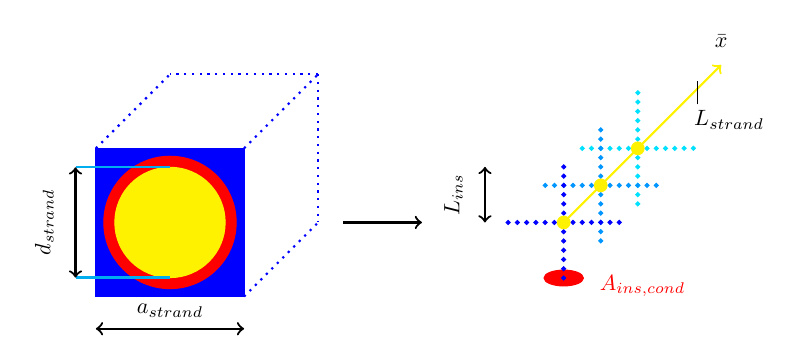
\begin{tikzpicture}[scale = 1]
        \filldraw[blue] (-0.941,-0.941) rectangle (0.941,0.941);
        \filldraw[red] (0,0) circle (0.7+0.07*2);
        \filldraw[yellow] (0,0) circle (0.7);
        \draw[thick, cyan] (-0.8*1.5,0.7) -- (0,0.7);
        \draw[thick, cyan] (-0.8*1.5,-0.7) -- (0,-0.7);
        \draw[black, thick, <->] (-0.75*1.6,0.7) -- (-0.75*1.6,-0.7);
        \node[scale = 0.8, rotate=90] at (-1.1*1.45, 0) {$d_\text{strand}$};
        \draw[thick,<->] (-0.941,-0.9*1.5) -- (0.941,-0.9*1.5);
        \node[scale = 0.8] at (0, -0.7*1.6) {$a_\text{strand}$};
        \draw[thick, dotted, blue] (0.941,0.941) -- (2*0.941,2*0.941);
        \draw[thick, dotted, blue] (-0.941,0.941) -- (0,2*0.941);
        \draw[thick, dotted, blue] (0.941,-0.941) -- (2*0.941,0);
        \draw[thick, dotted, blue] (2*0.941,2*0.941) -- (2*0.941,0);
        \draw[thick, dotted, blue] (2*0.941,2*0.941) -- (0,2*0.941);
        % ellipse for insulation area
        \filldraw[red] (5.0,-5.646/8) ellipse (0.25cm and 0.1cm);
        \node[scale = 0.8, red] at (6.0, -5.646/8-0.1) {$A_\text{ins,cond}$};
        % third insulation layer
        \definecolor{blue_third_layer}{RGB}{0,225,255}
        \foreach \x in {-5.646,-4.705,...,5.646} 
            \filldraw[blue_third_layer] (5.0+2*0.4705,\x/8+2*0.4705) circle (0.025);
        \foreach \x in {-5.646,-4.705,...,5.646} 
            \filldraw[blue_third_layer] (5.0+\x/8+2*0.4705,2*0.4705) circle (0.025);
        % second insulation layer
        \definecolor{blue_second_layer}{RGB}{0,150,255}
        \foreach \x in {-5.646,-4.705,...,5.646} 
            \filldraw[blue_second_layer] (5.0+0.4705,\x/8+0.4705) circle (0.025);
        \foreach \x in {-5.646,-4.705,...,5.646} 
            \filldraw[blue_second_layer] (5.0+\x/8+0.4705,0.4705) circle (0.025);
        % first insulation layer
        \definecolor{blue_first_layer}{RGB}{0,0,255}
        \foreach \x in {-5.646,-4.705,...,5.646} 
            \filldraw[blue_first_layer] (5.0,\x/8) circle (0.025);
        \foreach \x in {-5.646,-4.705,...,5.646} 
            \filldraw[blue_first_layer] (5.0+\x/8,0) circle (0.025);
        % strand nodes
        \draw[thick, yellow, ->] (5.0,0) -- (7.0,2.0);
        \foreach \t in {0.0,0.4705,...,1.4115}
            \filldraw[yellow] (5.0+\t,\t) circle (0.08);
        \node[scale = 0.8] at (7.1, 1.3) {$L_\text{strand}$};    
        \node[scale = 0.8] at (7, 2.3) {$\bar x$};    
        \draw[thin] (6.7,1.5) -- (6.7,1.8);
        \draw[thick, black, <->] (4,0) -- (4,5.646/8);
        \node[scale = 0.8, rotate=90] at (3.6, 5.646/16) {$L_\text{ins}$}; 
        % draw arrow
        \draw[thick, black, ->] (2.2,0) -- (3.2,0);
    \end{tikzpicture}
    \caption{3-dimensional transformation of a 1D+1D strand domain in ANSYS.}
    \label{fig: 1d_strand_geometry_with_insulation}
\end{figure}

In order to define the geometric parameters for the insulation layer with resin, one should calculate the insulation cross-sectional area as
\begin{equation}
    A_\text{ins} = a_\text{strand}^2 - \frac{\pi d_\text{strand}^2}{4}, 
    \label{eqn:cross_sectional_area_insulation}
\end{equation}
where $a_\text{strand}$ -- strand side, $d_\text{strand}$ -- strand diameter. Then, the average insulation perimeter is estimated as
\begin{equation}
    p_\text{avg} = \frac{4 a_\text{strand} + \pi d_\text{strand}}{2}.
    \label{eqn:average_perimeter}
\end{equation}
By combining the formulae (\ref{eqn:cross_sectional_area_insulation}) and (\ref{eqn:average_perimeter}), one can calculate the equivalent insulation length with resin as 
\begin{equation}
    L_\text{ins} = \frac{A_\text{ins}}{p_\text{avg}}.
    \label{eqn:equivalent_insulation_length}
\end{equation}
Calculating the equivalent insulation length with resin in such a manner allows for using this approximation also in case both the strand and the insulation are of the same shapes, e.g. if they are rectangles or circles. The conduction area of transverse elements is calculated as
\begin{equation}
    A_\text{ins, cond} = \frac{1}{4}~\frac{ A_\text{ins} ~ L_\text{strand} }{L_\text{ins}}~\frac{1}{n_\text{divisions, strand}},
    \label{eqn:equivalent_insulation_element_area}
\end{equation}
where $V_\text{ins}$ -- total insulation volume with resin, $n_\text{divisions, strand}$ -- number of divisions applied along the 1D strand domain. One should remember that $A_\text{ins, cond}$ of the insulation elements placed at two ends of the strand should be divided by two.~\cite{matthias_communication}

\subsection{Initial and Boundary Conditions, and Solver Settings}

The strand geometry, the temperature initial conditions, and the analysis settings for both COMSOL and ANSYS remain the identical with respect to the simulation described in Section~\ref{section: 1D_quench_propagation_no_insulation}, as presented in Fig. \ref{fig: init_gauss_temp_distr} and Table \ref{table: 1d_quench_propagation_analysis_init_temp_input_parameters}, respectively. The~analysis parameters are presented in Table \ref{table: 1d_quench_propagation_analysis_time_stepping_input_parameters}. The solver settings for both tools remain identical as well. The additional parameters corresponding to the insulation are described in Table~\ref{table: 1d_quench_propagation_geometry_parameters_with_insulation}. 

\begin{table}[H]
    \caption{Insulation input parameters.} 
    \vspace{-1.em} 
    \fontsize{10}{10}
    \selectfont 
    \renewcommand{\arraystretch}{1.5}
    \begin{center}
        \begin{tabular}{ ccc }
        \hline
        parameter & value & unit \\
        \hline
        $L_\text{ins}$ & 0.1679 & [mm] \\
        mesh size (insulation) & 28 & [\textmu m] \\
        \hline 
        \end{tabular}
    \end{center}  
     \label{table: 1d_quench_propagation_geometry_parameters_with_insulation} 
 \end{table}

Every orthogonal insulation domain consists of six elements of the same length. It is important to mention that in COMSOL, six orthogonal elements do not represent a quarter but a full cross-section. Therefore, the number of insulation elements in COMSOL is four times smaller and $A_\text{ins, cond}$ -- four times larger with respect to the analysis performed in ANSYS.

\subsection{Results}

Similarly to Section \ref{subsubsection:1d_quench_propagation_analysis_results_no_insulation}, the results are compared at three time steps, as presented in Fig. \ref{fig: 1d_with_insulation_temp_along_strand_comparison}. One can observe a slower quench propagation with time when the insulation is considered. At each time window, the hot-spot is placed at $x=0~\text{m}$.

\begin{figure}[H]
\centering
    \begin{tikzpicture}
        \begin{axis}[
          no markers,
          width=0.7\linewidth, 
          height = 5.0cm,
          xlabel={$\bar{x},~\text{m}$},
          ylabel={$T,~\text{K}$},
          xmin=0.0,
          ymin=0.0,
          xmax=1.0,
          legend pos=outer north east
          ]
        %   Initial temperature curve
          \addplot[smooth, black] table[x=posx,y=t_0_0_ans,col sep=comma] {sections/1D_quench_modelling/figures/results_with_insulation/10ms_1e4elemsf2_2ins_insTem_in.csv};
          
        %   COMSOL plots
          \addplot[smooth, red] table[x=posx,y=t_0_03_com,col sep=comma] {sections/1D_quench_modelling/figures/results_with_insulation/10ms_1e4elemsf2_2ins_insTem_in.csv};
          \addplot[smooth, red] table[x=posx,y=t_0_06_com,col sep=comma] {sections/1D_quench_modelling/figures/results_with_insulation/10ms_1e4elemsf2_2ins_insTem_in.csv};
          \addplot[smooth, red] table[x=posx,y=t_0_1_com,col sep=comma] {sections/1D_quench_modelling/figures/results_with_insulation/10ms_1e4elemsf2_2ins_insTem_in.csv};
        
        %   ANSYS plots
          \addplot[smooth, blue] table[x=posx,y=t_0_03_ans,col sep=comma] {sections/1D_quench_modelling/figures/results_with_insulation/10ms_1e4elemsf2_2ins_insTem_in.csv};
          \addplot[smooth, blue] table[x=posx,y=t_0_06_ans,col sep=comma] {sections/1D_quench_modelling/figures/results_with_insulation/10ms_1e4elemsf2_2ins_insTem_in.csv};
          \addplot[smooth, blue] table[x=posx,y=t_0_1_ans,col sep=comma] {sections/1D_quench_modelling/figures/results_with_insulation/10ms_1e4elemsf2_2ins_insTem_in.csv};
          
          \legend{
          $T_\text{init}$,
          COMSOL,,,
          ANSYS
          }

        \end{axis}
                  
        \draw[black, thick, ->] (1,3) -- (2,3);
        \node[scale = 1] at (2.8, 3) {$\vec{v}_\text{quench}$}; 
        
    \end{tikzpicture}
    \caption{Temperature distribution calculated in COMSOL and ANSYS for three time steps: $t=\{0.03, 0.06, 0.1\}$~s with a specified direction of the quench propagation, $\vec{v}_\text{quench}$.}
    \label{fig: 1d_with_insulation_temp_along_strand_comparison}
\end{figure}

The quench velocity is calculated by comparing the position of the quench front at $t=0.06~\text{s}$ and $t=0.1~\text{s}$. The relative error is calculated as in (\ref{eqn:relative_error_comsol_ansys_benchmarking}) and is estimated for: 
\begin{itemize}
    \item quench velocity, as presented in Table \ref{table: 1d_with_insulation_v_quench_comparison},
    \item temperature along the strand length at $t=0.1~\text{s}$, as presented in Fig. \ref{fig: ans_comsol_comparison_f_2_2_with_insulation}.
\end{itemize}

\begin{table}[H]
    \caption{Quench velocity comparison between COMSOL and ANSYS.} 
    \vspace{-1.em} 
    \fontsize{10}{10}
    \selectfont 
    \renewcommand{\arraystretch}{1.5}
    \begin{center}
        \begin{tabular}{ ccc }  
        \hline
        parameter & value & unit \\
        \hline
        $v_\text{quench, COMSOL}$ & 2.308 & [m/s] \\
        $v_\text{quench, ANSYS}$ & 2.310 & [m/s] \\
        $E_\text{r}$ & 0.108 & [\%] \\
        \hline 
        \end{tabular}
    \end{center}  
     \label{table: 1d_with_insulation_v_quench_comparison} 
 \end{table}

\begin{figure}[H]
\centering
    \begin{tikzpicture}
        \begin{axis}[
          width=0.7\linewidth, 
          height = 4.0cm,
          xlabel={$\bar{x},~\text{m}$},
          ylabel={$E_\text{r}$, \%},
          xmin=0.0,
          xmax=1.0
          ]
          \addplot[blue, mark=*] table[x=posx,y=error_0_1,col sep=comma] {sections/1D_quench_modelling/figures/results_with_insulation/10ms_1e4elemsf2_2ins_insTem_in_error.csv};
        \end{axis}
    \end{tikzpicture}
    \caption{Relative error along the strand with respect to the temperature distribution for $t=0.1~\text{s}$.}
    \label{fig: ans_comsol_comparison_f_2_2_with_insulation}
\end{figure}

The difference in quench velocity estimation in both models is less than 1\%, as presented in Table \ref{table: 1d_with_insulation_v_quench_comparison}. As shown in Fig. \ref{fig: 1d_with_insulation_temp_along_strand_comparison}, the relative error oscillates in the range of +2\% at the hot-spot to -2\% at the quench front. It means that ANSYS overestimates the hot-spot temperature and underestimates the temperature at the quench front with respect to COMSOL.

